% Options for packages loaded elsewhere
\PassOptionsToPackage{unicode}{hyperref}
\PassOptionsToPackage{hyphens}{url}
\documentclass[
  11pt,
]{article}
\usepackage{xcolor}
\usepackage[left=3cm,right=5cm,top=2cm,bottom=2cm]{geometry}
\usepackage{amsmath,amssymb}
\setcounter{secnumdepth}{5}
\usepackage{iftex}
\ifPDFTeX
  \usepackage[T1]{fontenc}
  \usepackage[utf8]{inputenc}
  \usepackage{textcomp} % provide euro and other symbols
\else % if luatex or xetex
  \usepackage{unicode-math} % this also loads fontspec
  \defaultfontfeatures{Scale=MatchLowercase}
  \defaultfontfeatures[\rmfamily]{Ligatures=TeX,Scale=1}
\fi
\usepackage{lmodern}
\ifPDFTeX\else
  % xetex/luatex font selection
\fi
% Use upquote if available, for straight quotes in verbatim environments
\IfFileExists{upquote.sty}{\usepackage{upquote}}{}
\IfFileExists{microtype.sty}{% use microtype if available
  \usepackage[]{microtype}
  \UseMicrotypeSet[protrusion]{basicmath} % disable protrusion for tt fonts
}{}
\makeatletter
\@ifundefined{KOMAClassName}{% if non-KOMA class
  \IfFileExists{parskip.sty}{%
    \usepackage{parskip}
  }{% else
    \setlength{\parindent}{0pt}
    \setlength{\parskip}{6pt plus 2pt minus 1pt}}
}{% if KOMA class
  \KOMAoptions{parskip=half}}
\makeatother
\usepackage{longtable,booktabs,array}
\newcounter{none} % for unnumbered tables
\usepackage{calc} % for calculating minipage widths
% Correct order of tables after \paragraph or \subparagraph
\usepackage{etoolbox}
\makeatletter
\patchcmd\longtable{\par}{\if@noskipsec\mbox{}\fi\par}{}{}
\makeatother
% Allow footnotes in longtable head/foot
\IfFileExists{footnotehyper.sty}{\usepackage{footnotehyper}}{\usepackage{footnote}}
\makesavenoteenv{longtable}
\usepackage{graphicx}
\makeatletter
\newsavebox\pandoc@box
\newcommand*\pandocbounded[1]{% scales image to fit in text height/width
  \sbox\pandoc@box{#1}%
  \Gscale@div\@tempa{\textheight}{\dimexpr\ht\pandoc@box+\dp\pandoc@box\relax}%
  \Gscale@div\@tempb{\linewidth}{\wd\pandoc@box}%
  \ifdim\@tempb\p@<\@tempa\p@\let\@tempa\@tempb\fi% select the smaller of both
  \ifdim\@tempa\p@<\p@\scalebox{\@tempa}{\usebox\pandoc@box}%
  \else\usebox{\pandoc@box}%
  \fi%
}
% Set default figure placement to htbp
\def\fps@figure{htbp}
\makeatother
% definitions for citeproc citations
\NewDocumentCommand\citeproctext{}{}
\NewDocumentCommand\citeproc{mm}{%
  \begingroup\def\citeproctext{#2}\cite{#1}\endgroup}
\makeatletter
 % allow citations to break across lines
 \let\@cite@ofmt\@firstofone
 % avoid brackets around text for \cite:
 \def\@biblabel#1{}
 \def\@cite#1#2{{#1\if@tempswa , #2\fi}}
\makeatother
\newlength{\cslhangindent}
\setlength{\cslhangindent}{1.5em}
\newlength{\csllabelwidth}
\setlength{\csllabelwidth}{3em}
\newenvironment{CSLReferences}[2] % #1 hanging-indent, #2 entry-spacing
 {\begin{list}{}{%
  \setlength{\itemindent}{0pt}
  \setlength{\leftmargin}{0pt}
  \setlength{\parsep}{0pt}
  % turn on hanging indent if param 1 is 1
  \ifodd #1
   \setlength{\leftmargin}{\cslhangindent}
   \setlength{\itemindent}{-1\cslhangindent}
  \fi
  % set entry spacing
  \setlength{\itemsep}{#2\baselineskip}}}
 {\end{list}}
\usepackage{calc}
\newcommand{\CSLBlock}[1]{\hfill\break\parbox[t]{\linewidth}{\strut\ignorespaces#1\strut}}
\newcommand{\CSLLeftMargin}[1]{\parbox[t]{\csllabelwidth}{\strut#1\strut}}
\newcommand{\CSLRightInline}[1]{\parbox[t]{\linewidth - \csllabelwidth}{\strut#1\strut}}
\newcommand{\CSLIndent}[1]{\hspace{\cslhangindent}#1}
\setlength{\emergencystretch}{3em} % prevent overfull lines
\providecommand{\tightlist}{%
  \setlength{\itemsep}{0pt}\setlength{\parskip}{0pt}}
\usepackage{amsmath,amsfonts,amssymb}
\usepackage{booktabs}
\usepackage{float}
\DeclareMathOperator{\Var}{Var}
\DeclareMathOperator{\Cov}{Cov}
\DeclareMathOperator{\Corr}{Corr}
\DeclareMathOperator{\tr}{tr}
\usepackage{bookmark}
\IfFileExists{xurl.sty}{\usepackage{xurl}}{} % add URL line breaks if available
\urlstyle{same}
\hypersetup{
  pdftitle={Power Analysis for Run-In Clinical Trials under AR(1) and General Correlation Structures},
  pdfauthor={Ronald G. Thomas},
  hidelinks,
  pdfcreator={LaTeX via pandoc}}

\title{Power Analysis for Run-In Clinical Trials under AR(1) and General
Correlation Structures}
\author{Ronald G. Thomas}
\date{April 20, 2026}

\begin{document}
\maketitle
\begin{abstract}
Paper 1 (Thomas, 2026) derived closed-form power formulas for
longitudinal trials with run-in and common close observations under
compound symmetry. The compound symmetry assumption implies that all
pairs of change scores are equally correlated, regardless of temporal
separation. In practice, observations closer in time are more strongly
correlated, and the AR(1) structure
\(\Corr(Y_{ijk}, Y_{ijk'}) = \rho^{|k-k'|}\) is a natural alternative.
We derive the variance of the treatment effect estimator under AR(1) via
two routes: (i) the Woodbury identity applied to the AR(1) marginal
covariance, and (ii) a moment-based approach using the cross-covariance
between run-in and treatment-period means. We characterize when the
efficiency gains from run-in designs are robust to the correlation
structure and when they depend sensitively on the exchangeability
assumption. A taxonomy of five correlation cases is developed, and
numerical comparisons use parameters from Alzheimer's disease
neuroimaging trials.
\end{abstract}

{
\setcounter{tocdepth}{2}
\tableofcontents
}
\section{Introduction}\label{introduction}

The efficiency of run-in designs depends on the correlation structure of
the repeated measurements. Under compound symmetry, the correlation
between any two change scores is constant, and the run-in observations
contribute information about the random slope \(b_i\) through a simple
averaging mechanism. Under AR(1), the correlation decays with temporal
separation, and the information content of run-in observations depends
on how far they are from the treatment period.

Paper 1 (\citeproc{ref-frost2008}{Frost et al. 2008}) assumed
\(R = \sigma^2(I_J +
\mathbf{1}_J\mathbf{1}_J')\), which arises from the change-score
parameterization under independent errors. Wang et al.
(\citeproc{ref-wang2019}{2019}) extended the run-in framework to
two-period linear mixed models but retained the compound symmetry
assumption. This paper extends to AR(1) residual correlation, where
\(\mathop{\mathrm{Corr}}(e_{ij}, e_{ij'}) =
\rho^{|j-j'|}\) for \(0 < \rho < 1\).

Winkens et al. (\citeproc{ref-winkens2007}{2007}) studied optimal
designs for autocorrelated longitudinal data but did not consider the
run-in setting. Diggle et al. (\citeproc{ref-diggle2002}{2002}) and
Verbeke and Molenberghs (\citeproc{ref-verbeke2000}{2000}) provide
general treatments of correlation structures in longitudinal models.
Chambless and Roeback (\citeproc{ref-chambless1993}{1993}) addressed the
effect of intra-individual variation on change-score analyses, a concern
that is amplified under AR(1) correlation.

The \texttt{longpower} R package (\citeproc{ref-iddi2022}{Iddi and
Donohue 2022}) is the CRAN reference implementation for
longitudinal-trial power calculations. Its closed-form routines
(\texttt{edland.linear.power()}, \texttt{diggle.linear.power()}) assume
random intercepts and slopes with independent or compound-symmetric
residuals, and the more flexible \texttt{liu.liang.linear.power()} and
\texttt{lmmpower()} accommodate arbitrary working covariances only
through simulation or a user-supplied fitted \texttt{lme} object. No
analytic AR(1)-residual formula is provided. The closed-form AR(1)
derivation developed here therefore fills a gap in the existing toolkit
while remaining consistent with the \texttt{longpower} formulae when the
correlation is replaced by its compound-symmetry limit.

\section{Correlation structures for longitudinal
trials}\label{correlation-structures-for-longitudinal-trials}

\subsection{Taxonomy of cases}\label{taxonomy-of-cases}

We consider five correlation structures for the raw outcomes
\(Y_{ijk}\):

\begin{enumerate}
\def\labelenumi{\arabic{enumi}.}
\item
  \textbf{Compound symmetry:}
  \(\mathop{\mathrm{Corr}}(Y_{ijk}, Y_{ijk'}) = \rho\) for all
  \(k \ne k'\). This is equivalent to the random intercept model and
  produces the \(R = \sigma^2(I +
  \mathbf{1}\mathbf{1}')\) structure in change scores.
\item
  \textbf{AR(1):}
  \(\mathop{\mathrm{Corr}}(Y_{ijk}, Y_{ijk'}) = \rho^{|k'-k|}\).
  Correlation decays geometrically with lag.
\item
  \textbf{Compound symmetry with variable run-in:} Case 1 with
  \(J_{0,i}\) varying across participants.
\item
  \textbf{AR(1) with variable run-in and common close:} Case 2 with
  \(J_{0,i}\) and \(J_{2,i}\) varying.
\item
  \textbf{General (unstructured):}
  \(\mathop{\mathrm{Corr}}(Y_{ijk}, Y_{ijk'}) = \sigma_{|k-k'|}/\sigma^2\).
\end{enumerate}

\subsection{Change-score correlations under each
structure}\label{change-score-correlations-under-each-structure}

Under the change-from-baseline parameterization (\(C_j = Y_j - Y_0\)),
the correlation between change scores depends on the raw-outcome
correlation structure.

For the run-in design with \(J_0 = 2\), \(J_1 = 1\):

\textbf{Compound symmetry:} \begin{align}
  \mathop{\mathrm{Corr}}(C_1, C_3) &= \frac{bt^2}{2a + bt^2} \\
  \mathop{\mathrm{Corr}}(C_1, C_2) &= \frac{-a + bt^2}{2a + bt^2}
\end{align}

\textbf{AR(1):} (to be derived)

\section{Variance under AR(1): GLS
approach}\label{variance-under-ar1-gls-approach}

\subsection{Marginal covariance}\label{marginal-covariance}

Under AR(1) with residual variance \(\sigma^2\) and autocorrelation
\(\rho\), the raw-outcome covariance is
\(\mathop{\mathrm{Cov}}(e_{ij}, e_{ij'}) = \sigma^2 \rho^{|j-j'|}\). The
change-score residual covariance becomes: \begin{equation}
  R_{jl} = \mathop{\mathrm{Cov}}(e_{ij} - e_{i0}, e_{il} - e_{i0})
  = \sigma^2(\rho^{|j-l|} - \rho^{|j|} - \rho^{|l|} + 1)
\end{equation} for \(j, l \ne 0\).

This \(R\) no longer has the rank-one-plus-identity structure, so the
Sherman-Morrison formula does not apply. However, the Woodbury identity
still reduces \(\Sigma^{-1}\) to a scalar inversion because \(G\)
remains scalar.

\subsection{Woodbury computation}\label{woodbury-computation}

The computation proceeds identically to Paper 1: \begin{equation}
  \Sigma^{-1} = R^{-1} - R^{-1}Z
    (G^{-1} + Z'R^{-1}Z)^{-1} Z'R^{-1}
\end{equation} with \(H = (G^{-1} + Z'R^{-1}Z)^{-1}\) still scalar. The
difference is that \(R^{-1}\) must be computed numerically (or via the
AR(1) tridiagonal inverse) rather than by Sherman-Morrison.

\begin{longtable}[]{@{}rrrrrr@{}}
\caption{Per-pair \(\mathop{\mathrm{Var}}(\hat\gamma)\) under AR(1) for
varying \(\rho\) (\(J_1=2\), \(J_2=0\), \(\sigma^2=1\),
\(\sigma_b^2=1\)).}\tabularnewline
\toprule\noalign{}
\(J_0\) & \(\rho=0\) & \(\rho=0.3\) & \(\rho=0.5\) & \(\rho=0.7\) &
\(\rho=0.9\) \\
\midrule\noalign{}
\endfirsthead
\toprule\noalign{}
\(J_0\) & \(\rho=0\) & \(\rho=0.3\) & \(\rho=0.5\) & \(\rho=0.7\) &
\(\rho=0.9\) \\
\midrule\noalign{}
\endhead
\bottomrule\noalign{}
\endlastfoot
0 & 3.0000 & 2.9100 & 2.7500 & 2.5100 & 2.1900 \\
2 & 2.1569 & 2.0132 & 1.6662 & 1.1157 & 0.3963 \\
4 & 1.3268 & 1.3902 & 1.2218 & 0.8508 & 0.3036 \\
\end{longtable}

\section{Variance under AR(1): moment-based
approach}\label{variance-under-ar1-moment-based-approach}

\subsection{Cross-covariance between phase
means}\label{cross-covariance-between-phase-means}

An alternative to the GLS approach computes the variance of the pre-post
test statistic directly from the moments of the phase means. Let
\(\bar{X}_0 = \frac{1}{J_0}\sum_{i=1}^{J_0} Y_{i,\text{run-in}}\) and
\(\bar{X}_K = \frac{1}{J_1}\sum_{j=1}^{J_1} Y_{j,\text{trt}}\) denote
the run-in and treatment-period means.

Under AR(1) with parameter \(c = \rho\), the cross-covariance is:
\begin{equation}
  \mathop{\mathrm{Cov}}(\bar{X}_0, \bar{X}_K)
  = \frac{\sigma^2}{J_0 c}\,\rho_1\, c^{K-1}\,
    \frac{(1 - c^{J_0})(1 - c^{J_1})}{(1 - c)^2}
\end{equation} where \(K\) is the gap between the last run-in and first
treatment observation.

\subsection{Variance of the change
score}\label{variance-of-the-change-score}

The variance of the pre-post difference is: \begin{equation}
  \mathop{\mathrm{Var}}(X_K - X_0) = \mathop{\mathrm{Var}}(X_K) + \mathop{\mathrm{Var}}(X_0)
    - 2\mathop{\mathrm{Cov}}(X_K, X_0)
\end{equation}

The variance of each phase mean involves the sum
\(S_n = \sum_{i=1}^{n-1}(n-i)c^{i-1}\), which has the closed form:
\begin{equation}
  S_n = \frac{n(1-c) - (1-c^n)}{(1-c)^2}
\end{equation}

\begin{verbatim}
## Moment-based vs GLS variance (r=2, k=2, rho=0.5):
\end{verbatim}

\begin{verbatim}
##   Moment-based (sigma_b=0): 1.4375
\end{verbatim}

\begin{verbatim}
##   GLS (sigma_b=1.0):       1.6662
\end{verbatim}

\begin{verbatim}
##   (Moment-based ignores random slope.)
\end{verbatim}

\section{Relationship between the two
approaches}\label{relationship-between-the-two-approaches}

The GLS approach (Section 3) and the moment-based approach (Section 4)
compute different quantities. The GLS variance is the minimum-variance
bound under the assumed model, while the moment-based variance is the
variance of the simple averaged change-score estimator
\(\bar{d}_1 - \bar{d}_0\).

When \(\sigma_b^2 = 0\) (no random slope), the two approaches coincide
because the GLS estimator reduces to the simple difference of means.
When \(\sigma_b^2 > 0\), the GLS estimator is strictly more efficient
because it uses the full covariance structure \(\Sigma = R + ZGZ'\) to
weight the observations optimally, while the moment-based approach
treats all observations within a phase equally.

The practical value of the moment-based computation is that it provides
a conservative (upper) bound on the variance under AR(1) without
requiring specification of \(\sigma_b^2\). The ratio of the two
variances quantifies the efficiency loss from ignoring the random slope
structure -- this is the relative efficiency studied in Paper 4.

\section{Robustness to correlation
misspecification}\label{robustness-to-correlation-misspecification}

The practical question is whether a trial designed under compound
symmetry loses substantial efficiency when the true correlation is
AR(1), and vice versa.

\begin{figure}
\centering
\pandocbounded{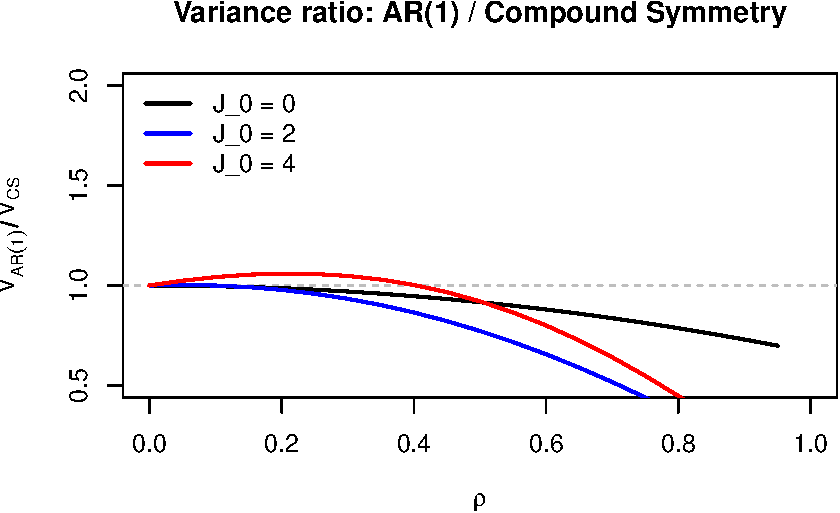
\includegraphics[keepaspectratio,alt={Ratio of AR(1) to compound symmetry variance as a function of \textbackslash rho for three run-in configurations (J\_1=2, J\_2=0, \textbackslash sigma\^{}2=1, \textbackslash sigma\_b\^{}2=1).}]{report_files/report_files/figure-latex/robustness-1.pdf}}
\caption{Ratio of AR(1) to compound symmetry variance as a function of
\(\rho\) for three run-in configurations (\(J_1=2\), \(J_2=0\),
\(\sigma^2=1\), \(\sigma_b^2=1\)).}
\end{figure}

\section{Stratified variance for unequal visit
patterns}\label{stratified-variance-for-unequal-visit-patterns}

When participants have different numbers of run-in (\(J_{0,i}\)) or
common close (\(J_{2,i}\)) observations, the total variance is a
weighted sum across strata: \begin{equation}
  \frac{1}{n^2}\sum_{s=1}^{S} n_s\,
    \mathop{\mathrm{Var}}(X_K - X_0)\big|_{J_0 = J_{0,s},\, J_2 = J_{2,s}}
\end{equation}

\section{Numerical examples}\label{numerical-examples}

\subsection{Comparison across correlation
structures}\label{comparison-across-correlation-structures}

\begin{longtable}[]{@{}rrrrr@{}}
\caption{Sample size per group (MIRIAD parameters, \(\Delta=0.25\), 90\%
power) under compound symmetry vs AR(1).}\tabularnewline
\toprule\noalign{}
\(J_0\) & \(J_1\) & \(J_2\) & \(N\) (CS) & \(N\) (AR(1),
\(\rho=0.5\)) \\
\midrule\noalign{}
\endfirsthead
\toprule\noalign{}
\(J_0\) & \(J_1\) & \(J_2\) & \(N\) (CS) & \(N\) (AR(1),
\(\rho=0.5\)) \\
\midrule\noalign{}
\endhead
\bottomrule\noalign{}
\endlastfoot
0 & 2 & 0 & 329 & 328 \\
1 & 2 & 0 & 3 & 2 \\
2 & 2 & 0 & 2 & 1 \\
3 & 2 & 0 & 1 & 1 \\
4 & 2 & 0 & 1 & 1 \\
\end{longtable}

\subsection{Sensitivity to rho}\label{sensitivity-to-rho}

\begin{figure}
\centering
\pandocbounded{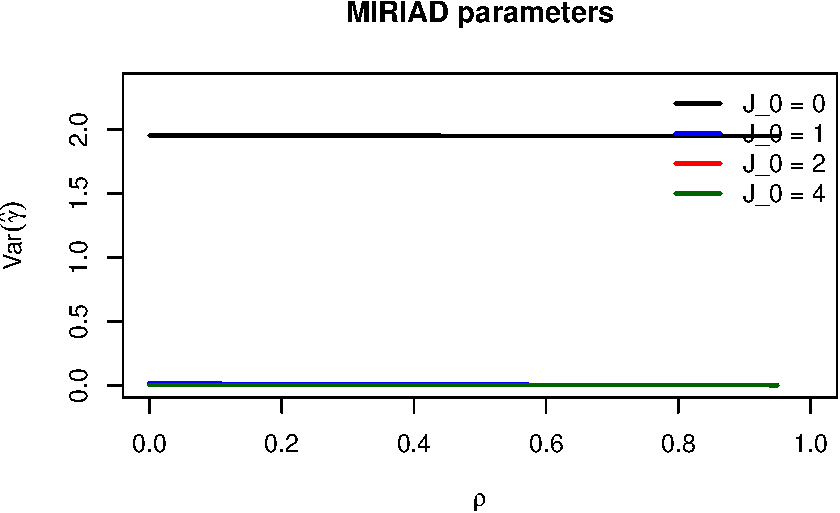
\includegraphics[keepaspectratio,alt={Per-pair variance as a function of \textbackslash rho under AR(1) for MIRIAD parameters (\textbackslash sigma\^{}2=0.0025, \textbackslash sigma\_b\^{}2=0.9745, J\_1=2, J\_2=0).}]{report_files/report_files/figure-latex/sensitivity-1.pdf}}
\caption{Per-pair variance as a function of \(\rho\) under AR(1) for
MIRIAD parameters (\(\sigma^2=0.0025\), \(\sigma_b^2=0.9745\),
\(J_1=2\), \(J_2=0\)).}
\end{figure}

\section{Discussion}\label{discussion}

\section*{References}\label{references}
\addcontentsline{toc}{section}{References}

\protect\phantomsection\label{refs}
\begin{CSLReferences}{1}{1}
\bibitem[\citeproctext]{ref-chambless1993}
Chambless, Lloyd E., and Joellen R. Roeback. 1993. {``Methods for
Assessing Difference Between Groups in Change When Initial Measurement
Is Subject to Intra-Individual Variation.''} \emph{Statistics in
Medicine} 12 (14): 1213--37.
\url{https://doi.org/10.1002/sim.4780121403}.

\bibitem[\citeproctext]{ref-diggle2002}
Diggle, Peter J., Patrick Heagerty, Kung-Yee Liang, and Scott L. Zeger.
2002. \emph{Analysis of Longitudinal Data}. 2nd ed. Oxford University
Press.

\bibitem[\citeproctext]{ref-frost2008}
Frost, Chris, Michael G. Kenward, and Nick C. Fox. 2008. {``Optimizing
the Design of Clinical Trials Where the Outcome Is a Rate. {Can}
Estimating a Baseline Rate in a Run-in Period Increase Efficiency?''}
\emph{Statistics in Medicine} 27 (18): 3717--31.
\url{https://doi.org/10.1002/sim.3280}.

\bibitem[\citeproctext]{ref-iddi2022}
Iddi, Samuel, and Michael C. Donohue. 2022. {``Power and Sample Size for
Longitudinal Models in {R} -- the Longpower Package and {Shiny} App.''}
\emph{The R Journal} 14 (1): 264--82.
\url{https://journal.r-project.org/articles/RJ-2022-022/}.

\bibitem[\citeproctext]{ref-verbeke2000}
Verbeke, Geert, and Geert Molenberghs. 2000. \emph{Linear Mixed Models
for Longitudinal Data}. Springer.

\bibitem[\citeproctext]{ref-wang2019}
Wang, Guoqiao, Andrew J. Aschenbrenner, Yan Li, et al. 2019.
{``Two-Period Linear Mixed Effects Models to Analyze Clinical Trials
with Run-in Data When the Primary Outcome Is Continuous: {Applications}
to {Alzheimer's} Disease.''} \emph{Alzheimer's \& Dementia:
Translational Research \& Clinical Interventions} 5: 450--57.
\url{https://doi.org/10.1016/j.trci.2019.08.002}.

\bibitem[\citeproctext]{ref-winkens2007}
Winkens, Bjorn, Gerard J. P. van Breukelen, Hubert J. A. Schouten, and
Martijn P. F. Berger. 2007. {``Randomized Clinical Trial Designs for
Auto-Correlated Longitudinal Data.''} \emph{Statistics in Medicine} 26
(28): 5023--37. \url{https://doi.org/10.1002/sim.2907}.

\end{CSLReferences}

\end{document}
